\documentclass[11pt,letterpaper]{article}
\usepackage{fullpage}
\usepackage[pdftex]{graphicx}
\usepackage{amsfonts,eucal,amsbsy,amsopn,amsmath}
\usepackage{url}
\usepackage[sort&compress]{natbib}
\usepackage{natbibspacing}
\usepackage{latexsym}
\usepackage{wasysym} 
\usepackage{rotating}
\usepackage{fancyhdr}
\DeclareMathOperator*{\argmax}{argmax}
\DeclareMathOperator*{\argmin}{argmin}
\usepackage{sectsty}
\usepackage[dvipsnames,usenames]{color}
\usepackage{multicol}
\definecolor{orange}{rgb}{1,0.5,0}
\usepackage{multirow}
\usepackage{sidecap}
\usepackage{caption}
\renewcommand{\captionfont}{\small}
\setlength{\oddsidemargin}{-0.04cm}
\setlength{\textwidth}{16.59cm}
\setlength{\topmargin}{-0.04cm}
\setlength{\headheight}{0in}
\setlength{\headsep}{0in}
\setlength{\textheight}{22.94cm}
\allsectionsfont{\normalsize}
\newcommand{\ignore}[1]{}
\newenvironment{enumeratesquish}{\begin{list}{\addtocounter{enumi}{1}\arabic{enumi}.}{\setlength{\itemsep}{-0.25em}\setlength{\leftmargin}{1em}\addtolength{\leftmargin}{\labelsep}}}{\end{list}}
\newenvironment{itemizesquish}{\begin{list}{\setcounter{enumi}{0}\labelitemi}{\setlength{\itemsep}{-0.25em}\setlength{\labelwidth}{0.5em}\setlength{\leftmargin}{\labelwidth}\addtolength{\leftmargin}{\labelsep}}}{\end{list}}

\bibpunct{(}{)}{;}{a}{,}{,}
\newcommand{\nascomment}[1]{\textcolor{blue}{\textbf{[#1 --NAS]}}}


\pagestyle{fancy}
\lhead{}
\chead{}
\rhead{}
\lfoot{}
\cfoot{\thepage~of \pageref{lastpage}}
\rfoot{}
\renewcommand{\headrulewidth}{0pt}
\renewcommand{\footrulewidth}{0pt}


\title{11-712:  NLP Lab Report}
\author{Jesse Dodge}
\date{April 25, 2014}

\begin{document}
\maketitle
\begin{abstract}
In this paper we approach the problem of dependency parsing for French. We discuss some relevant aspects of the French language, and examine previous work on this problem. After describing some available resources such as tools for tokenization datasets in French, we present our approach for dependency parsing French. First, taking a supervised approach, we present results training TurboParser, a high-speed, high-accuracy parser. Second, we show that adding features from semi-supervised Brown clusters gives a significant improvement. Finally, we discuss self-training using a large corpus of unannotated text. 
\end{abstract}

\section{Basic Information about French}
French is a Roman language, spoken in many countries around the world. It's the 10th most commonly spoken language in the world, with between 220 and 300 million people speaking French as a first or second language. French is spoken as a first language in France, Haiti, and Monaco, and in parts of Switzerland, the United States, and Canada, . Roughly half of the French speaking population of the world live in Europe, but many also live in African countries such as Gabon, Mauritius, Algeria, Senegal, and Côte d'Ivoire. French was a language of trade and diplomacy from the 17th century to the middle of the 20th century, until English came into prominence. Today, it still is used by many international organizations, such as NATO, Red Cross, and Amnesty International. \\
For it's writing system, French uses the 26 characters in the Latin alphabet plus a number of diacritical marks. There are two grammatical genders in French, and a number of past, present, and future tenses (some of which are formed with auxiliary verbs). French is a subject-verb-object language, and has both active and passive voice (like English).

\section{Past Work on the Syntax of French}
French syntax has been well studied. There exist texts ranging from simple (e.g. Fundamentals of French Syntax\footnote{http://www.academia.edu/1997083/Fundamentals\_of\_French\_Syntax}) to complex (e.g. The Syntax of French\footnote{http://www.amazon.com/Syntax-French-Cambridge-Guides/dp/B008SLJ1WQ}, Foundations of French Syntax\footnote{http://www.amazon.com/Foundations-French-Cambridge-Textbooks-Linguistics/dp/0521388058}). Beyond just textbooks, there are a number of papers that address individual topics in French such as verb movement\footnote{http://minimalism.linguistics.arizona.edu/AMSA/PDF/AMSA-175-1000.pdf} and tokenization\footnote{https://giguete.users.greyc.fr/pricai96/part4.html}.

With repsect to syntax for parsing, there exists a French constituency-parsed treebank$\footnote{http://alpage.inria.fr/statgram/frdep/fr\_stat\_dep\_parsing.html}$ which contains 12,531 sentenecs from Le Monde, a French newspaper annotated with morphology, phrase-structure, and grammatical functions that has been converted into dependency trees\footnote{http://alpage.inria.fr/statgram/frdep/fr\_stat\_dep\_parsing.html}. This resource has some annotation guidelines, but they're somewhat limited and in French. In this work, we followed these guidelines as closely as possible, and where they were lacking, found similar guidelines for English. Where there was no help from the guidelines and the languages diverged, we created a set of rules and documented them. 

\section{Available Resources}
As one of the most spoken languages in the world, there is a tremendous amount of available text in French, from French news articles to French Wikipedia to French literature. In this work, we will focus on Europarl\footnote{http://www.statmt.org/europarl/}, a parallel corpus of 21 languages of transcriptions of court cases. Europarl has 194 MB corpus of French-English text. We present two test datasets, A and B, which we annotated on the first one thousand and second one thousand words of Europarl, respectively. \\
Part of speech (PoS) tagging is also a task that has been approached before. From the treebank, two PoS taggers were found to have been trained. TreeTagger\footnote{http://www.cis.uni-muenchen.de/~schmid/tools/TreeTagger/}, an open-source part of speech tagger, and Stanford's PoS tagger with a French model. In this work, Stanford's tagger was used, which gives coarse part of speech tags. \\
Tokenization in French is a difficult problem, and two systems were compared qualitatively. First, Europarl comes packaged with a  tokenization tool, and second Stanford's PoS tagger has tokenization built in. When compared, Stanford's tokenizer was found to be inferior to the rule-based tool from Europarl. As an example, consider the following sentence:
\begin{center}
Qu'est-ce qu'il y a? (What's the matter?)
\end{center}
In sentences like these, where either a question word (or phrase) is used or the inversion is used, there are often contractions or hyphenations. These cues were mostly ignored by Stanford's system, leading to the following tokenization:
\begin{center}
\begin{tabular}{c|c|c|c}
Qu'est-ce & qu'il & y & a \\
\end{tabular}
\end{center}
On the other hand, the Europarl tool often over-tokenized, splitting almost every place there was found any punctuation, leading to the following tokenization:
\begin{center}
\begin{tabular}{c|c|c|c|c|c}
Qu'& est-ce & qu'& il & y & a \\
\end{tabular}
\end{center}
Arguably, this question is formed of two multi-word expressions, so the correct tokenization should simply be:
\begin{center}
\begin{tabular}{c|c}
Qu'est-ce qu'& il y a \\
\end{tabular}
\end{center}
\section{Survey of Phenomena in French}
In this section, we will focus on the relevant phenomena in French for dependency parsing. Much French syntax and grammar is similar to that of English, and so won't be covered in great depth. 
\subsection{Negation}
Negation in French has two parts. For example, the sentence \textit{Je suis riche} (\textit{I am rich}) is negated as \textit{Je \textbf{ne} suis \textbf{pas} riche}. (\textit{I am \textbf{not} rich}). The \textit{pas} from the example can be replaced with \textit{jamais} to mean \textit{never}, or with \textit{rien} to mean \textit{nothing}, etc.
\subsection{Auxiliaries}
Auxiliary verbs are often used in a number of tenses, such as the pass\'{e} compos\'{e} (the most common past tense). For example \textit{j'\textbf{ai} mangé cinq fois hier} (\textit{I ate five times yesterday}) contains the auxiliary \textit{\textbf{ai}}. These function in a similar way to English. 
\subsection{The inversion}
When asking a question in French, one can either use question words at the begging of the sentence (such as \textit{Qu'est-ce que}) or use the inversion, where you invert the order of the verb and either its subject or object. Again, this is similar to English.
\subsection{Reflexive verbs}
While both French and English have reflexive verbs, they are far more common in French. For example, the sentence \textit{Vous \textbf{vous} levez tard} translates literally to \textit{You get \textbf{yourself} up late}, where the reflexive pronoun is in bold.
\subsection{Register}
French contains six registers\footnote{http://french.about.com/od/lessons/a/register.htm}, or levels of formality. The most formal French is typically only written. In this work, we're examining court proceedings, which are formal in register. In more formal French registers, idiomatic expressions and formality-indicating phrases (which are often semantically vacuous) appear often.
\subsection{Grammatical gender}
Nouns in French have gender, and French pronouns are based on the gender of the noun they are associated with. Similarly, determiners and possessive adjectives agree with the nouns they qualify. 

\section{Initial Design}
For the initial design of the dependency parser, we trained TurboParser \footnote{https://www.ark.cs.cmu.edu/TurboParser/}, a fully supervised dependency parser. TurboParser is a nonprojective dependency parser that uses up to third-order features for grand-siblings and tri-siblings, and has state-of-the-art performance on English dependency parsing. Our training data consisted of 1,000 tokens of French Europarl annotated with unlabeled dependency trees and coarse PoS tags. For this experiment, we used the default settings on TurboParser, and tested on test set A (another 1,000 tokens of annotated French Europarl). 

\section{System Analysis on Corpus A}
The initial design lead to an accuracy of 56.7\%. When analyzing the errors, it became evident that a significant portion of the errors came from the annotations of punctuation. During annotation, punctuation characters that were marked as tokens by the Europarl tokenizer were somewhat arbitrarily added to the dependency tree, leading to very low scores on punctuation during test. The reference guidelines on dependency parsing in French had no information on punctuation. \\ 

\section{Lessons Learned and Revised Design}
It is clear that having consistent and logical annotation rules is beneficial. Additionally, the training dataset is quite small; increasing the size of the training set almost always leads to an increase in performance. The results of the initial design show that having a small training corpus can make training a high-quality model difficult. This begs the question: Can we take advantage of the large amount of unannotated text when learning to generate dependency parses? 
\subsection{Additional annotations}
Another 1,000 tokens were annotated to add to the training set, from the same corpus.
\subsection{Annotation revisions}
For each sentence in the training and test corpora, the annotation of the punctuation was revised. The final punctuation of the sentence became a child of the head of the sentence. Similarly, commas, when denoting a subordinate clause became children of the head of the parent clause. Commas in lists (first, second, and third) were annotated as children of the head of the list. Quotation marks were annotated as the children of the head of tokens they were surrounding. Finally, apostrophes, when used in contractions, became the children of the left-most word of the contraction. In French apostrophes are often used when a word ends in a vowel and the following word starts with a vowel, as in \textit{Que est-ce que il y a} $\rightarrow$ \textit{Qu'est-ce qu'il y a}. 
\subsection{Brown clusters}
Brown clustering\footnote{http://acl.ldc.upenn.edu/J/J92/J92-4003.pdf} is an unsupervised approach for clustering words. Brown clustering has been shown to help with a number of NLP applications, including dependency parsing\footnote{http://www.cs.columbia.edu/~mcollins/papers/koo08acl.pdf}. The Brown clustering algorithm takes a set of sentences (the corpus) as input and returns a hierarchical clustering of the words in the corpus. Each word belongs to one cluster, and the hierarchy can be seen as a tree. See Figure 1 for an example. \\
\begin{figure}[t!]
    \centering
    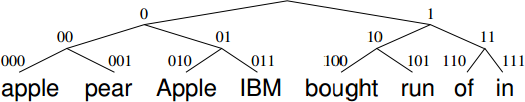
\includegraphics[width=0.6\textwidth]{images/brown_clusters.png}
    \caption{An example Brown brown clustering for a small vocabulary.}
    \label{fig:brown}
\end{figure}
The only parameter to the Brown clustering algorithm is the number of clusters. For this work, we tried 25, 50, and 100 clusters. \\

\section{System Analysis on Corpus B}
In this section, we analyze the results of the improvements described in section 7.
\subsection{Additional annotations}
The additional 1,000 training tokens added to the training set increased accuracy to 66.2\%.
\subsection{Annotation revisions}
Punctuation makes up around 10\% of the corpus, so we saw significant gains from revisiting the annotations. These revisions boosted the accuracy to 76\%. 
\subsection{Brown clusters}
These experiments were run with the corrected training data set of 2,000 tokens. 
\begin{center}
\begin{tabular}{|c|c|}
\hline
Number of clusters & Accuracy\\
\hline
25 & 77.7\%\\
50& 77.8\%\\
100 & \textbf{78}\%\\
\hline
\end{tabular}
\end{center}
These results show that the Brown clusters helped significantly, netting a 2\% absolute accuracy boost.

\section{Final Revisions}
As expected, the unsupervised features helped. To try to take further advantage of the large amount of unannotated data available, a self-training approach was used. 
\subsection{Self-training}
Self-training has been shown to be useful when dealing with a limited amount of labeled training data but presented with a large amount of unlabeled data. Below is pseudocode for the self-training algorithm used in this work.
\begin{enumerate}
\item Train the parser on the hand-annotated training data.
\item Using the trained parser, predict trees on a set of unannotated sentences. 
\item Using the union of the predicted trees and the hand-annotated training data, retrain the parser.
\item Run the parser on the test set.
\end{enumerate}
Multiple rounds of self-training have, in the past, been found to hurt because of semantic drift\footnote{Curran et al.,
2007}; therefore, only one round of self-training was used. Results are presented below. 
\begin{center}
\begin{tabular}{|c|c|}
\hline
Number of additional training tokens & Accuracy\\
\hline
2,000 & 76.6\%\\
4,000 & 76.8\%\\
10,000 & \textbf{78}\%\\
20,000 & 77.4\%\\
50,000 & 77.7\%\\
100,000 & 76.6\%\\
500,000 & 77.1\%\\
\hline
\end{tabular}
\end{center}
As we can see, in most cases the self-training didn't help performance, and only matched performance on the set of size 10,000. 

\section{Future Work}
This worked focused on contrasting supervised and semi-supervised learning for dependency parsing. However, much work has gone into both of these topics, and additional performance can be gleaned from building upon what others have done in the past. Morphological features (such as lemmatization) have been shown to increase performance, though it's possible some of the information gained through these features is already captured in the Brown clusters. Syntactic features specific to the French language (i.e. those not already built in to TurboParser) are another candidate for future work. Of course, increasing the size of the training set would give a sure gain. 

\label{lastpage}
\end{document}
